\documentclass[12pt,a4paper]{article}
\usepackage[utf8]{inputenc}
\usepackage{polski}
\usepackage[polish]{babel}
\usepackage{amsmath}
\usepackage{amsfonts}
\usepackage{amssymb}
\usepackage{graphicx}
\usepackage[export]{adjustbox}
\usepackage{wrapfig}
\usepackage{caption}
\usepackage{adjustbox}

\numberwithin{equation}{section}

\renewcommand{\baselinestretch}{1.5}
\captionsetup[figure]{labelformat={default},name={\bfseries Rys.}}
\captionsetup[table]{labelformat={default},name={\bfseries Tab.}}

\newcommand*{\captionsource}[2]{%
	\caption[{#1}]{%
		#1%
		\\\hspace{\linewidth}%
		\textbf{Żródło:} #2%
	}%
}


\title{2. Mostek Wheatstone'a}
\date{25 października 2017}	
\author{
	Zespół 3: Górski Paweł, Sozańska Ada\\
	EAIiIB Informatyka, Rok II
}

\begin{document}
\maketitle
% WPROWADZENIE
\section{Wprowadzenie}
Celem tego doświadczenia jest wyznaczenie nieznanych oporów oraz zweryfikowanie wzorów na opór zastępczy oporników w połączeniach: szeregowym i równoległym, przy wykorzystaniu praw Kirchhoffa oraz prawa Ohma.

\subsection{Prawa Kirchhoffa, prawo Ohma}

Mostek Wheatstone'a jest oparty na trzech fundamentalnych prawach obwodów elektrycznych.

Pierwszym z nich jest \emph{Prądowe Prawo Kirchhoffa}. Dotyczy ono prądów wpływających do węzła obwodu elektrycznego oraz mówi, że suma algebraiczna prądów wpływających do danego węzła jest równa zeru. Zakładając, że do węzła wpływa $n$ prądów $I_j$, gdzie $j \in \{1,2,~\ldots,~n\}$, prawo to można zapisać następująco:
\begin{equation}
	\sum_{j = 1}^{n} I_j = 0.
	\label{krichoff1}
\end{equation}

\pagebreak
Kolejnym prawem jest \emph{Napięciowe Prawo Kirchhoffa}, które dotyczy spadków napięć w oczku (zamkniętej pętli sieci) obwodu elektrycznego. Mówi ono, że suma spadków napięć na wszystkich elementach w oczku jest równa zeru. Zakładając, że w oczku jest $n$ elementów elektrycznych, prawo to można zapisać następująco:
\begin{equation}
	\sum_{j = 1}^{n} U_j = 0.
	\label{krichoff2}
\end{equation}

Ostatnim prawem jest \emph{Prawo Ohma}, które definiuje zależność natężenia i napięcia prądu. Mówi ono, że stosunek napięcia $U$ między końcami przewodnika do natężenia prądu $I$ w nim płynącego jest wielkością stałą. Wielkość ta jest nazywana opornością. 
\begin{equation}
	R = \frac{U}{I}.
	\label{ohm}
\end{equation}
Prawo to może nie być spełnione w elementach nieliniowych (np. dioda) lub gdy temperatura przewodnika nie jest stała.

\pagebreak
\subsection{Mostek Wheatstone'a}

Mostek Wheatstone'a jest układem do porównywania oporów. Oprócz pomiaru wielkości typowych dla obwodów elektrycznych jest on również wykorzystywany do budowania mierników naprężeń, ciśnień hydrostatycznych czy próżni. 

\begin{figure}[!htb]
	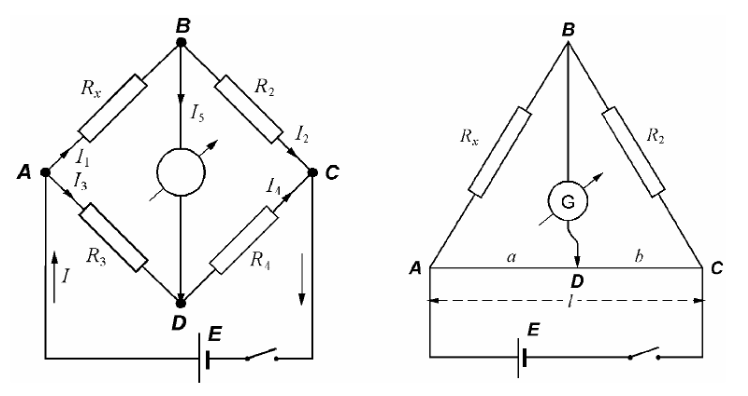
\includegraphics[width=1\textwidth]{img/mostek.png} 
	\captionsource{Schemat mostka Wheatstone'a. Niezrównoważony (po lewej) oraz zrównoważony (po prawej).}{Instrukcja do ćwiczenia}
	\label{fig:img1}
\end{figure}


Składa się on z czterech oporników o oporach: $R_x, R_2, R_3, R_4$ oraz galwanometru o oporze $R_5$. Stosując \emph{Prądowe Prawo Kirchhoffa} (\ref{krichoff1}) dla węzłów $B, D$ otrzymujemy następujące równania:
\begin{equation}
	\begin{split}
	&B:~I_1 = I_2 + I_5, \\
	&D:~I_5 = I_3 - I_4.
	\end{split}
	\label{eq:e1}
\end{equation}

\pagebreak
Następnie wykorzystując \emph{Napięciowe Prawo Kirchhoffa} (\ref{krichoff2}) dla oczek $ABDA, BCDB$ otrzymujemy dwa równania:
\begin{equation}
	\begin{split}
	ABDA:&~I_1 R_x + I_5 R_5 - I_3 R_3 = 0, \\
	BCDB:&~I_2 R_2 - I_4 R_4 - I_5 R_5 = 0.
	\end{split}
	\label{eq:e2}
\end{equation}

W doświadczeniu wykorzystujemy układ zrównoważony, w którym potencjały w węzłach $B$ i $D$ są równe. W konsekwencji mamy $I_5 = 0$~A, co powoduje uproszczenie układu równań (\ref{eq:e1}) do:
\begin{equation}
	\begin{split}
	I_1 = I_2, \\
	I_3 = I_4.
	\end{split}
\end{equation}
Dalej, równania (\ref{eq:e2}) upraszczają się do postaci:
\begin{equation}
	\begin{split}
	I_1 R_x = I_3 R_3 , \\
	I_1 R_2 = I_3 R_4.
	\end{split}
\end{equation}
Co nam daje:
\begin{equation}
	R_x = R_2\frac{R_3}{R_4}.
	\label{eq:e3}
\end{equation}

W mostku zrównoważonym opory $R_3$ oraz $R_4$ są oporami wewnętrznymi przewodów o długości kolejno $a$ oraz $b = l - a$ (Rys. \ref{fig:img1}). Opory te można przedstawić wzorami:
\begin{equation}
		R_3 = \rho\frac{a}{S}~~\textrm{oraz}~~R_4 = \rho \frac{l - a}{S},
		\label{eq:e4}
\end{equation}
gdzie $\rho$ to oporność właściwa, a $S$ to pole przekroju wewnętrznego przewodu.

Ostatecznie, korzystając z (\ref{eq:e3}) i (\ref{eq:e4}) otrzymujemy wzór, w którym wszystkie parametry są mierzalne:
\begin{equation}
	R_x = R_2 \frac{a}{l - a}.
	\label{eq:rx}
\end{equation}

\pagebreak
% WYKONANIE ĆWICZENIA
\section{Wykonanie ćwiczenia}
\label{sec:2}


W celu wykonania doświadczenia wykorzystaliśmy:
\begin{itemize}
	\item Listwę o długości $1$~m z podziałką milimetrową, drutem oporowym i suwakiem,
	\item Opornicę dekadową $R_2$,
	\item Zestaw pięciu oporników $R_x$,
	\item Mikroamperomierz,
	\item Zasilacz stabilizowany $3$~A/$30$~V.
\end{itemize}

Doświadczenie rozpoczęliśmy od połączenia elementów w zrównoważony mostek Wheatstone'a. Suwak na listwie przesunęliśmy do połowy jej długości ($a = 50$~cm). Dla każdego z pięciu oporników $R_x$ ustawialiśmy opór $R_2$ na opornicy dekadowej tak, aby amperomierz wskazywał $0$~A. Następnie osiem razy zmienialiśmy opór $R_2$, żeby oscylował w okół wartości początkowej $R_2$ (ustawionej dla $a = 50$~cm) i dostosowywaliśmy suwak, tak aby za każdym razem amperomierz wskazywał $0$ A.

Analogiczne pomiary wykonaliśmy dla połączenia szeregowego (opory $R_{x1}$ i $R_{x2}$), równoległego (opory $R_{x1}$ i $R_{x2}$) i mieszanego (opór $R_{x3}$ szeregowo z równolegle połączonymi oporami $R_{x1}$ i $R_{x2}$).

\pagebreak
% OPRACOWANIE DANYCH POMIAROWYCH
\section{Opracowanie danych pomiarowych}
\subsection{Pomiary}
W poniższej tabeli prezentujemy wyniki pomiarów dla każdego opornika. Pomiary zostały wykonane tak, jak opisano to w sekcji \emph{Wykonanie ćwiczenia}. Opór $R_x$ każdego z oporników został obliczony ze wzoru (\ref{eq:rx}) dla $l = 1000$~mm (długość całego drutu), oraz dla wartości $a$ i $R_2$ podanych w tabeli.

\begin{table}[!ht]
	\caption{Wartości pomiarów nieznanych oporów $R_x$}
	\begin{adjustbox}{width=1\textwidth}
		\begin{center}
			\begin{tabular}{l||c|c|c|c|c|c|c|c|c}
				\multicolumn{10}{c}{\bfseries Opornik 1} \\ \hline
				$R_2$ [$\Omega$] & 8,2 & 9,2 & 10,2 & 11,2 & 12,2 & 13,2 & 14,2 & 15,2 & 16,2 \\
				$a$ [mm] & 599 & 572 & 550 & 522 & 500 & 482 & 465 & 450 & 431 \\
				$R_{x1}$ [$\Omega$] & 12,249 & 12,295 & 12,467 & 12,231 & 12,200 & 12,283 & 12,342 & 12,436 & 12,271 \\ \hline
				\multicolumn{10}{c}{\bfseries Opornik 2} \\ \hline
				$R_2$ [$\Omega$] & 31,1 & 32,1 & 33,1 & 34,1 & 35,1 & 36,1 & 37,1 & 38,1 & 39,1 \\
				$a$ [mm] & 530 & 521 & 514 & 507 & 500 & 492 & 483 & 476 & 470 \\
				$R_{x2}$ [$\Omega$] & 35,070 & 34,915 & 35,007 & 35,068 & 35,100 & 34,963 & 34,660 & 34,610 & 34,674 \\ \hline
				\multicolumn{10}{c}{\bfseries Opornik 3} \\ \hline
				$R_2$ [$\Omega$] & 62,0 & 64,0 & 66,0 & 68,0 & 70,0 & 72,0 & 74,0 & 76,0 & 78,0 \\
				$a$ [mm] & 527 & 519 & 511 & 503 & 500 & 494 & 487 & 481 & 474 \\
				$R_{x3}$ [$\Omega$] & 69,07 & 69,05 & 68,96 & 68,82 & 70,00 & 70,29 & 70,25 & 70,43 & 70,28 \\ \hline
				\multicolumn{10}{c}{\bfseries Opornik 4} \\ \hline
				$R_2$ [$\Omega$] & 35,8 & 36,8 & 37,8 & 38,8 & 39,8 & 40,8 & 41,8 & 42,8 & 43,8 \\
				$a$ [mm] & 527 & 519 & 513 & 506 & 500 & 494 & 487 & 481 & 475 \\
				$R_{x4}$ [$\Omega$] & 39,887 & 39,707 & 39,818 & 39,743 & 39,800 & 39,832 & 39,681 & 39,666 & 39,629 \\ \hline
				\multicolumn{10}{c}{\bfseries Opornik 5} \\ \hline
				$R_2$ [$\Omega$] & 72,7 & 82,7 & 92,7 & 102,7 & 112,7 & 122,7 & 132,7 & 142,7 & 152,7 \\
				$a$ [mm] & 608 & 577 & 548 & 520 & 500 & 481 & 461 & 443 & 419 \\
				$R_{x5}$ [$\Omega$] & 112,76 & 112,81 & 112,39 & 111,26 & 112,70 & 113,72 & 113,50 & 113,49 & 110,12 \\ \hline
			\end{tabular}
		\end{center}
	\end{adjustbox}
	\label{tab:tab1}
\end{table}

Dla każdego opornika policzyliśmy średnią arytmetyczną z dziewięciu wyznaczonych wartości oporów zawartych w tabeli (Tab. \ref{tab:tab1}). Następnie obliczyliśmy niepewność standardową pomiarów, korzystając z estymatora odchylenia standardowego średniej tych wyników. Wyniki przedstawiliśmy w tabeli poniżej.

\begin{table}[!ht]
	\caption{Średnie arytmetyczne oporów $R_x$ oraz ich niepewności $u(R_x)$}
	\begin{center}
		\begin{tabular}{l||c|c|c|c|c}
			\hline
			$L,p,$ & 1 & 2 & 3 & 4 & 5 \\ \hline
			$R_x$ [$\Omega$] & 12,308 & 34,896 & 69,68 & 39,751 & 112,53  \\
			$u(R_{x})$ [$\Omega$] & 0,030 & 0,065 & 0,22 & 0,029 & 0,38 \\ \hline
		\end{tabular}
	\end{center}
	\label{tab:tab2}
\end{table}

W tabeli poniżej znajdują się analogiczne pomiary dla połączenia szeregowego (opory $R_{x1}$ i $R_{x2}$), równoległego (opory $R_{x1}$ i $R_{x2}$) i mieszanego (opór $R_{x3}$ szeregowo z równolegle połączonymi oporami $R_{x1}$ i $R_{x2}$).

\begin{table}[!ht]
	\caption{Wartości pomiarów nieznanych oporów dla różnych połączeń}
	\begin{adjustbox}{width=1\textwidth}
		\begin{center}
			\begin{tabular}{l||c|c|c|c|c|c|c|c|c}
				\multicolumn{10}{c}{\bfseries Połączenie szeregowe} \\ \hline
				$R_2$ [$\Omega$] & 39,5 & 41,5 & 43,5 & 45,5 & 47,5 & 49,5 & 51,5 & 53,5 & 55,5 \\
				$a$ [mm] & 547 & 535 & 523 & 512 & 500 & 489 & 472 & 463 & 454 \\
				$R_{szer}$ [$\Omega$] & 47,69 & 47,74 & 47,69 & 47,73 & 47,50 & 47,36 & 46,03 & 46,12 & 46,14 \\ \hline
				\multicolumn{10}{c}{\bfseries Połączenie równoległe} \\ \hline
				$R_2$ [$\Omega$] & 5,5 & 6,5 & 7,5 & 8,5 & 9,5 & 10,5 & 11,5 & 12,5 & 13,5 \\
				$a$ [mm] & 631 & 587 & 555 & 524 & 500 & 474 & 449 & 427 & 409 \\
				$R_{row}$ [$\Omega$] & 9,405 & 9,238 & 9,353 & 9,357 & 9,500 & 9,462 & 9,371 & 9,315 & 9,342 \\ \hline
				\multicolumn{10}{c}{\bfseries Połączenie mieszane} \\ \hline
				$R_2$ [$\Omega$] & 72,0 & 74,0 & 76,0 & 78,0 & 80,0 & 82,0 & 84,0 & 86,0 & 88,0 \\
				$a$ [mm] & 526 & 520 & 513 & 506 & 500 & 494 & 487 & 481 & 476 \\
				$R_{miesz}$ [$\Omega$] & 79,899 & 80,167 & 80,057 & 79,895 & 80,000 & 80,055 & 79,743 & 79,703 & 79,939 \\ \hline
			\end{tabular}
		\end{center}
	\end{adjustbox}
	\label{tab:tab3}
\end{table}

Następnie obliczyliśmy średnią arytmetyczną z wyników w tabeli \mbox{(Tab. \ref{tab:tab3})} oraz niepewności pomiarów tych wyników. Dodatkowo, poniżej zawarliśmy obliczone wartości oporów zastępczych w tych konfiguracjach oraz ich niepewności złożone, korzystając z wyników zawartych w tabeli (\mbox{Tab. \ref{tab:tab2}}).

\begin{table}[!ht]
	\caption{Średnie arytmetyczne oporów $R$ oraz ich niepewności $u(R)$ dla różnych połączeń}
	\begin{center}
		\begin{tabular}{l||c|c|c}
			\multicolumn{4}{c}{\bfseries Mierzone} \\ \hline
			Połączenie & Szeregowe &  Równoległe & Mieszane \\ \hline
			$R_{mierz}$ [$\Omega$] & 47,11 & 9,371 & 79,939 \\
			$u(R_{mierz})$ [$\Omega$] & 0,25 & 0,025 & 0,050 \\ \hline
			\multicolumn{4}{c}{\bfseries Obliczone} \\ \hline
			Połączenie & Szeregowe &  Równoległe & Mieszane \\ \hline
			$R_{oblicz}$ [$\Omega$] & 47,204 & 9,098 & 78,77 \\
			$u(R_{oblicz})$ [$\Omega$] & 0,071 & 0,016 & 0,22 \\ \hline
		\end{tabular}
	\end{center}
	\label{tab:tab4}
\end{table}

W celu obliczenia wartości oporów zastępczych dla rozważanych w doświadczeniu połączeń wykorzystaliśmy następujące wzory, wynikające z praw Kirchhoffa:
\begin{align}
	& R_{szer} = R_1 + R_2, \label{eq:r1} \\
	& R_{row} = \frac{R_1 R_2}{R_1 + R_2}, \label{eq:r2} \\
	& R_{miesz} = \frac{R_1 R_2}{R_1 + R_2} + R_3. \label{eq:r3}
\end{align}


Dla połączenia szeregowego wykorzystaliśmy wzór (\ref{eq:r1}), do połączenia równoległego wzór (\ref{eq:r2}), a do połączenia mieszanego wzór (\ref{eq:r3}) (będący konsekwencją użycia dwóch poprzednich wzorów).


Niepewności dla obliczonych wartości oporów zastępczych wyliczyliśmy ze wzorów wynikających z prawa przenoszenia niepewności oraz powyższych równań:
\begin{equation}
\small
\begin{split}
u(R_{szer}) &= \sqrt{u(R_1)^2 + u(R_2)^2}, \\
u(R_{row}) &= \sqrt{\Bigg(\frac{R_2^2}{(R_1 + R_2)^2} u(R_1)\Bigg)^2 + \Bigg(\frac{R_1^2}{(R_1 + R_2)^2} u(R_2)\Bigg)^2}, \\
u(R_{miesz}) &= \sqrt{\Bigg(\frac{R_2^2}{(R_1 + R_2)^2} u(R_1)\Bigg)^2 + \Bigg(\frac{R_1^2}{(R_1 + R_2)^2} u(R_2)\Bigg)^2 + u(R_3)^2}.
\end{split}
\end{equation}

\subsection{Analiza wyników}

Analizując dane zawarte w tabeli (Tab. \ref{tab:tab4}) jesteśmy w stanie sprawdzić zgodność między wartościami zmierzonymi, a obliczonymi dla różnych konfiguracji połączeń oporników.

Dla połączenia szeregowego: 
\begin{equation}
	\begin{split}
	& R_{mierz} = 47,11~\Omega,~~~~R_{oblicz} = 47,204~\Omega, \\
	& \Delta R = \Big| R_{mierz} - R_{oblicz} \Big| = 0,094~\Omega, \\
	& U(\Delta R) = 2 \sqrt{u(R_{mierz})^2 + u(R_{oblicz})^2} = 0,52~\Omega. \\
	\end{split}
\end{equation}

Wartości mierzona oraz obliczona dla połączenia szeregowego są zgodne, gdyż $\Delta R = 0,094~\Omega < U(\Delta R) = 0,52~\Omega$.

Dla połączenia równoległego: 
\begin{equation}
\begin{split}
& R_{mierz} = 9,371~\Omega,~~~~R_{oblicz} = 9,098~\Omega, \\
& \Delta R = \Big| R_{mierz} - R_{oblicz} \Big| = 0,27~\Omega, \\
& U(\Delta R) = 2 \sqrt{u(R_{mierz})^2 + u(R_{oblicz})^2} = 0,060~\Omega. \\
\end{split}
\end{equation}

Wartości mierzona oraz obliczona dla połączenia równoległego okazują się być niezgodne, gdyż $\Delta R = 0,27~\Omega > U(\Delta R) = 0,060~\Omega$.

Dla połączenia mieszanego: 
\begin{equation}
\begin{split}
& R_{mierz} = 79,939~\Omega,~~~~R_{oblicz} = 78,77~\Omega, \\
& \Delta R = \Big| R_{mierz} - R_{oblicz} \Big| = 1,169~\Omega, \\
& U(\Delta R) = 2 \sqrt{u(R_{mierz})^2 + u(R_{oblicz})^2} = 0,45~\Omega. \\
\end{split}
\end{equation}

Wartości mierzona oraz obliczona dla połączenia mieszanego nie są zgodne, gdyż $\Delta R = 1,169~\Omega > U(\Delta R) = 0,45~\Omega$.

\section{Wnioski}

Z analizy wartości zmierzonych i obliczonych oporów zastępczych jesteśmy w stanie potwierdzić prawdziwość wzoru na opór zastępczy dla połączenia szeregowego, ponieważ wyniki są ze sobą zgodne w granicach błędu.

Niestety dla połączeń równoległego oraz mieszanego wyniki nie były ze sobą zgodne. Mogło to wynikać z faktu, iż założyliśmy, że opornica dekadowa ma pomijalnie mały błąd. Wpływ na ten wynik mógł mieć również stan okablowania, ponieważ nie wszystkie przewody dało się stabilnie przyłączyć do elementów układu elektrycznego, co wiązało się z fałszowaniem wyników wskazywanych przez amperomierz.


\end{document}